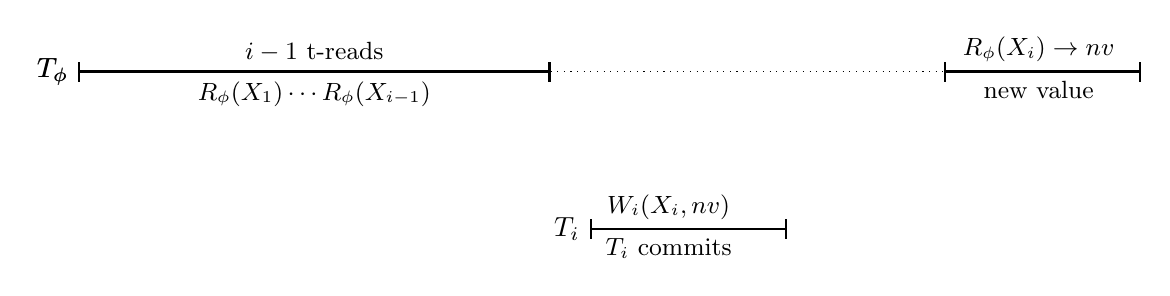
\begin{tikzpicture}
\node (r1) at (3,0) [] {};
%\node (r2) at (7.7,0) [] {};
\node (r3) at (12.2,0) [] {};

%\node (w1) at (7.5,-2) [] {};

\node (w2) at (7.5,-2) [] {};

\draw (r1) node [below] {\small {$R_{\phi}(X_1) \cdots R_{\phi}(X_{i-1})$}};
\draw (r1) node [above] {\small {$i-1$ t-reads}};

\draw (w2) node [above] {\small {$W_{i}(X_{i},nv)$}}; 
\draw (w2) node [below] {\small {$T_{i}$ commits}};

\draw (r3) node [above] {\small {$R_{\phi}(X_{i})\rightarrow nv$}};
\draw (r3) node [below] {\small {new value}};


\begin{scope}   
\draw [|-|,thick] (0,0) node[left] {$T_{\phi}$} to (6,0);
\draw [|-|,dotted] (0,0) node[left] {$T_{\phi}$} to (13.5,0);
\draw [|-|,thick] (11,0) node[left] {} to (13.5,0);
\end{scope}
%
%
\begin{scope}   
%\draw [|-|,thick] (0,0) node[left] {$T_k$} to (6,0);
\draw [|-|,thick] (6.5,-2) node[left] {$T_i$} to (9,-2);
\end{scope}
%
\end{tikzpicture}
%